\documentclass{article} % Jean-C�me Charpentier 2006
\usepackage{graphicx}
\usepackage{pst-all}
\usepackage[a4paper]{geometry}

\begin{document}

\begin{pspicture}(-2,0)(12,10)
  \rput(0,4){\makebox[0pt][l]{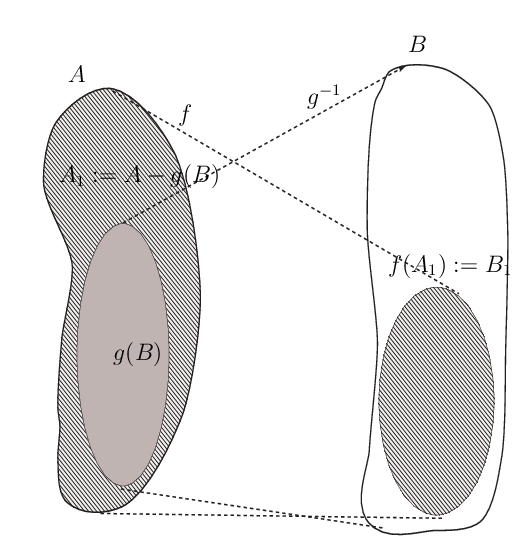
\includegraphics[width=10cm]{supfyg}}}
% image tiger is available on CTAN or your TeX installation
%  \psgrid[griddots=10,subgriddiv=0]
  \psset{linewidth=1pt,arrows=<-}
  \rput(1,7.25){$A$}
  \rput(6,7.25){$B$}
  \rput(3,6.25){$f$}
  \rput(5,6.25){$g^{-1}$}
  \rput(1,5){$A_1:=A-g(B)$}
  \end{pspicture}
  
  
  
  
  

\end{document}